\documentclass[conference]{IEEEtran}

\usepackage{graphicx}
\DeclareGraphicsExtensions{.pdf,.jpg,.png}
\graphicspath{{./figs/} {./plots/}}

\usepackage{balance}
\usepackage{comment}
\usepackage{xspace}
\usepackage[export]{adjustbox}
\usepackage{wrapfig}
\usepackage{multicol}
\usepackage{float}
\newcommand{\sys}{Safewalk\xspace}
\author{
  \IEEEauthorblockN{
   Iljoo Baek, Mengwen He and Emily Ruppel
  }
 \IEEEauthorblockA{
   Carnegie Mellon University
  }
 \IEEEauthorblockA{
   {ibaek,mengwenhe,eruppel}@andrew.cmu.edu
  }
}
\title{Gait Monitoring using Wireless Sensors\\
        \vspace{4mm}
        \large{Final Report 18-748}\\
        \large{Spring 2017}}

\begin{document}

\maketitle

%Only including an abstract since it looks like the submission site wants one... 
\begin{abstract}
Killer abstract. 
\end{abstract}

\section{Introduction}
  \label{sec:intro}
  Gait patterns, the measurable characteristics of an individual’s walking movement, can
provide insight into a variety of components of an individual’s health status. Certain
gait pathologies may be associated with specific medical conditions. Sudden changes in the
way an individual walks can be indicative of the occurrence of an undetected but
deleterious medical event, i.e. undetected stroke. A shift in gait pattern over time may
come about as the result of muscular or neural decline that could increase the probability
of a dangerous event, such as a fall, in the future. However, diagnosing conditions or
predicting an increased fall risk from gait patterns requires the attention of a trained
medical professional, which limits the settings in which gait analysis can be used.
    
Wireless Body Area Networks have been proposed as a promising solution for capturing
useful health status indicators without inconveniencing a patient~\cite{wban}. The
additional data enables a new field of computer-assisted physical therapy that allows
therapists to deliver more targeted care to their patients. Advanced treatment centers for
patients with unique cases, such as the Walter Reed Center for Performance and Clinical
Research (CPCR) amputee clinic, use extensive computer modeling to aid in patient
rehabilitation~\cite{cpcr}.  An apparent barrier to the widespread adoption of computer
assisted therapy is the cost of the motional analysis systems. For instance, the CPCR uses
23 infrared cameras to track the movement of reflective markers attached to a patient's
body and six force plates in the floor to fully capture a patient's movement. Though the
movement data can be captured and used at a later time, the gait analysis is still limited
to a clinical setting. 
  
Our project's goal was to expand the usefulness of gait analysis beyond a professional’s
office to an individual’s day-to-day environment. We accomplished our goal by
demonstrating a proof-of-concept gait monitoring system that relies on wireless motes
instrumented with Inertial Measurement Units (IMUs) to capture relevant data and relay
them to a powerful backend machine for offline and real time processing. Our system
extracted a variety of components of the subject's gait pattern from linear and angular
acceleration data measured at specfic points along his or her legs. The subject's
movements were then visualized and features of the gait were plotted in real time. We also
demonstrate the practicality of real-time fall detection by using a simple thresholding
technique to indicate when a subject is no longer upright. Throughout the trials with our
prototype system we note that wireless sensor networks are particularly promising for
accomplishing gait detection because the small nodes and lack of constraining wires
minimizes the impact on the patient and allows for an honest gait assessment without the
residual impact of cumbersome measurement devices. 
%
%Add note about final system architecture in Intro... should make the technical
%description easier and it still make sense to do that here
%
\section{Related Work}
This project is based on prior work in gait assessment, IMU data interpretation, and
wireless communication. In this section we will describe how the prior work influenced the
design of our project 

\section{Technical Description}
To implement our gait monitoring system we had to handle three major design points-
transmitting data from the IMUs, analyzing the IMU data, and building a useful interface
to the information. This section will describe the choices our team made with regards to
these three subsystems. 
\subsection{Device Communication}
Moving data from the IMU to the remote server can be separated into two distinct
transitions-- one from IMU to firefly slave device and another from the slave to the
master node. As shown in Figure~\ref{fig:ff}, the IMU board attaches directly to the
Firefly. The connection provides power from the Firefly batteries to the IMU and allows
for two way communication over one of the Firefly's auxiliary UART ports and the
configurable IMU communication ports. The majority of the data transported over the serial
connection is the IMU readings transported from the IMU board to the Firefly whenever the
IMU has data available. 

\begin{figure}[ht]
  \centering
  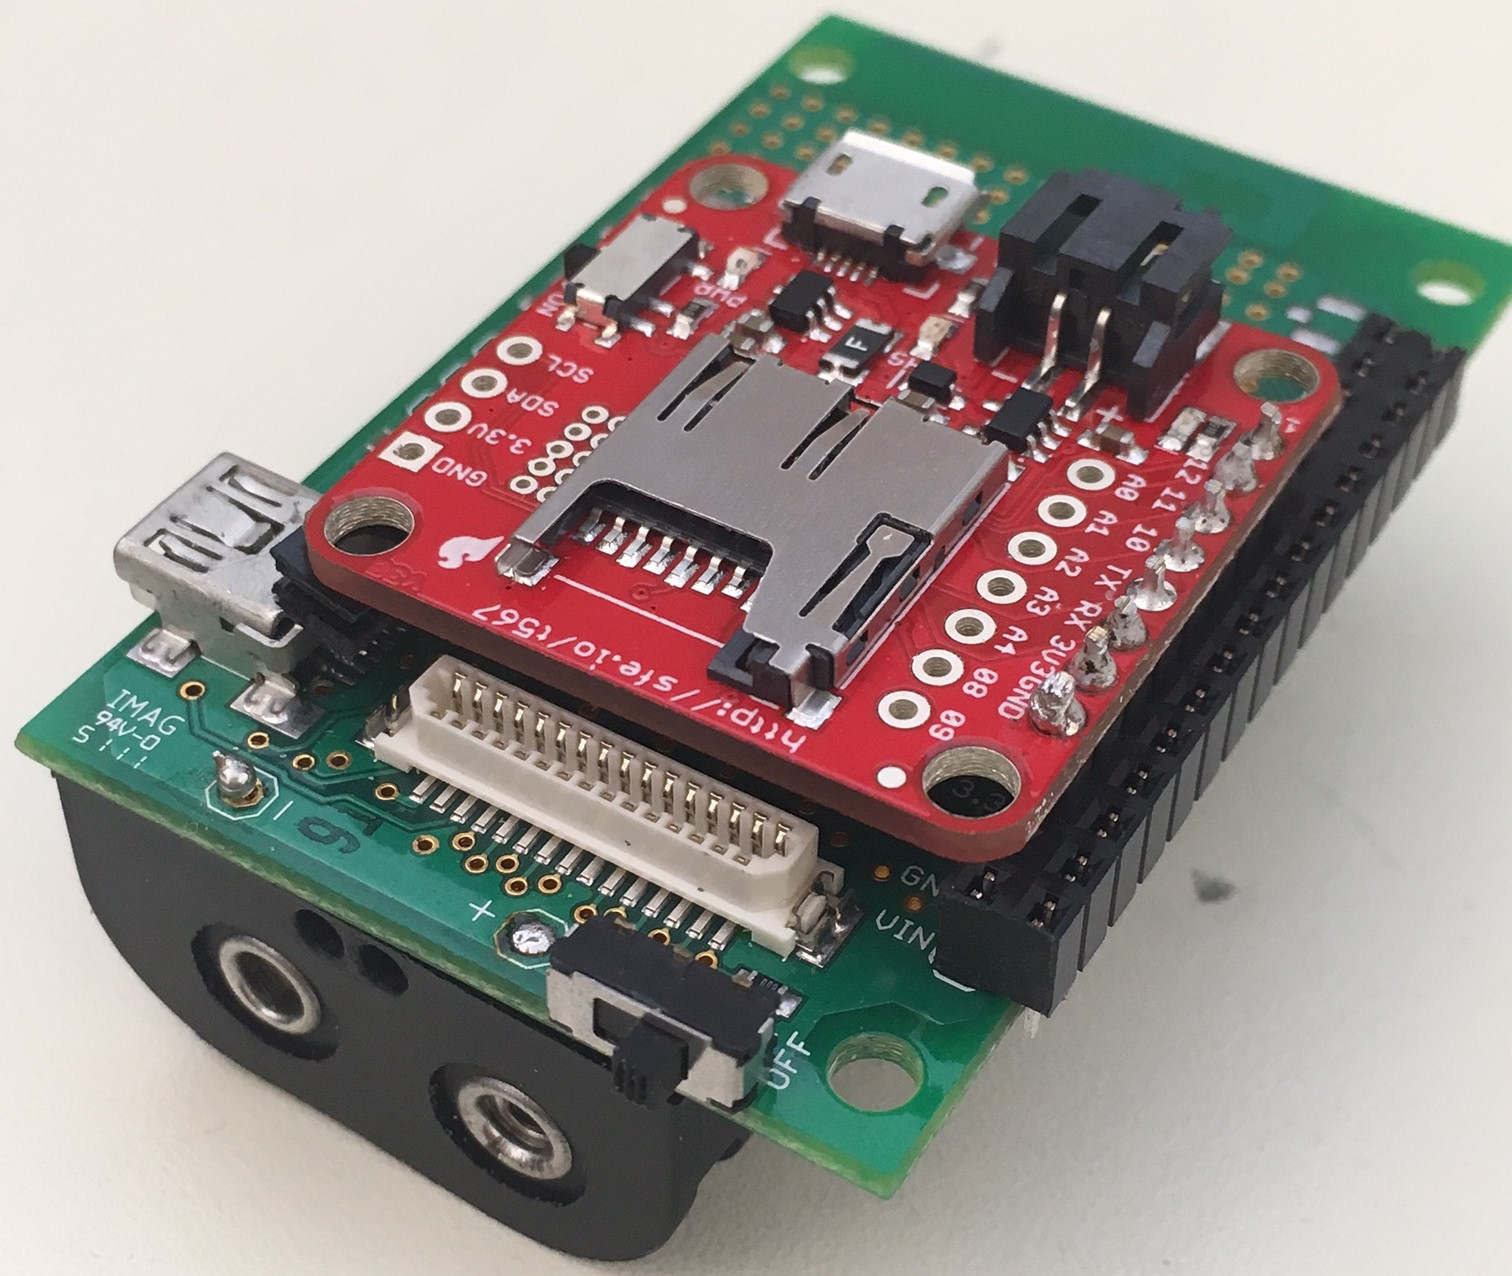
\includegraphics[width=0.8\columnwidth]{figs/cropped2}
  \caption{{\bf Firefly node with IMU board attached}}
  \label{fig:ff}
\end{figure}

  The format of the packet passed from IMU to Firefly is shown in
Figure ~\ref{fig:packet}. The data are encoded as ASCII characters to simplifiy debugging
as data move from IMU to firefly slave node to master and final output. While the ASCII
encoding greatly simplified debugging, it does mean that the packet size may change given
different accelerometer values.  Throughout the project, several unsuccessful attempts
were made to tightly control the data transmission by the IMU board, but the nature of the
UART protocol made timing discrepancies between the two devices difficult to overcome, and
was further complicated by the variable packet size. Instead, we settled on a four
character pattern to indicate the beginning of an IMU transmission followed by a single
special character to indicate the end. In contrast to the long packets transmitted from
the IMU board, the firefly needs only to issue commands to the IMU, so the protocol from
firefly to IMU is far simpler. If the IMU board receives a character from the Firefly, the
corresponding command is retrieved from a look-up table and carried out. A final feature
of the IMU-Firefly communication protocol is automatic reboot of the firefly. 
  Once packets are passed from the IMU to the Firefly slave device, the firefly transmits
the packet using the Point Coordination Function (PCF) TDMA protocol~\cite{pcf}. Each
slave device is statically assigned a time slot according to its preprogrammed MAC address
and only transmits during its assigned slot. The PCF TDMA protocol is designed for a
network with a star topology, where all slave nodes are within one hop of the master
device because all slave nodes must synchronize based on a message sent from the master at
the beginning of every TDMA cycle.  Despite its simplicity, this protocol met our design
goals of maximizing data throughput by preventing collisions without inucurring the time
overhead of carrier sense~\cite{CSMA}.  During its designated time slot, a slave node
transmits the packet passed to it from the IMU after stripping off the start and stop
bytes. An added advantage of the TDMA protocol is the implicit ID and time information
coupled with each transmission. Based on the time slot during which a packet is received,
the master node can automatically attach the ID of the node that transmitted the packet
before passing the entire packet to the server for processing. Further, the time
synchronization as a result of TDMA allows for the assumption that the measurements from
different IMUs received during a given TDMA cycle occurred at the same time. Therefore,
the server can afix a timestamp to data based on when it receives the data rather than
transmitting a timestamp from the slave node indicating the precise moment when the IMU
measurement was made. 

The protocol delivers a data rate of approximately 10 packets per second from each of
the slave nodes. This rate could be improved by decreasing the packet size, and more
tightly matching the TDMA slot length to the transmission time of a packet. In the current
configuration, the slot length is fixed at 10ms per node. Further exploration of the
transmit and receive task lengths on the slave nodes could also improve throughput.
Currently both the receive and transmit tasks operate on a period of 250ms. In the
transmit task, a slave device transmits as many times as possible given the tdma protocol
before switching to the receive task, but during the receive task the node will receive a
message with low probability because the master sends commands to the slaves infrequently.
Reducing the length of the receive period will thererfore reduce the slave node's idle
time with little impact on the system's performance. 

  The only command transmitted from the master to the slaves beyond the TDMA synchronization
is a "Recalibrate" command that signals the slave nodes to send messages to their IMUs to
perform static calibration. This command is sent only when a users pushes the auxiliary
button the master firefly at the beginning of a long period of system operation. While the
communication protocol is complicated by this single command, it is important that the
master node be able to issue a synchronous recalibration command to all of the nodes to
improve the accuracy of the following measurements. The recalibraton phase samples the
baseline static noise floor of each IMU, so the subject wearing the devices must be
stationary while the devices are undergoing recalibration. It is difficult for the subject
to remain stationary if each of the devices must be manually turned off and then on to initiate
recalibration. The master's recalibrate command circumvents the issue by causing all IMUs
to recalibrate instantaneously which greatly reduces the amount of time the patient must
remain still. 

\subsection{Gait Analysis}

\subsection{User Interface}

\section{Results}
Add picture of final enclosure. Discuss how it was attached to the subject. Mention that
it was fairly stable.

Talk about all of the calculations and provide examples from data we have lying around. 

\section{Conclusion} 


\balance
\bibliographystyle{abbrv}
\bibliography{sigproc}  % sigproc.bib is the name of the Bibliography in this case
\end{document}

